\documentclass[12pt]{article}

\usepackage{sbc-template}
\usepackage{caption}
\usepackage{subcaption}
\usepackage{float}

\usepackage{graphicx,url}

\usepackage[brazil]{babel}   
%\usepackage[latin1]{inputenc}  
\usepackage[utf8]{inputenc}  
% UTF-8 encoding is recommended by ShareLaTex

     
\sloppy

\title{Replicação de Processos}

\author{Marlon Henry Schweigert\inst{1},Jonathan de Oliveira Cardoso\inst{1}}


\address{Centro de Ciências Tecnológicas -- Universidade do Estado de Santa Catarina (UDESC)\\
Joinville -- Santa Catarina -- Brasil
  \email{\{marlon.henry,jonathan.cardoso\}@edu.udesc.br}
}

\begin{document} 

\maketitle
     
\begin{resumo} 
  Este artigo descreve a construção do serviço para resolução de empacotamento de pesos utilizando tolerância a falhas entre os processos, com mecanismos de lockstep, recovery e health.
\end{resumo}


\section{Replicação}

A replicação de processos é um ponto crucial para o funcionamento de sistemas de alta disponibilidade. Grandes empresas atuais utilizam dessa abordagem para tratar grandes problemas de escalabilidade utilizando replicação de dados e processos.

Ter um sistema altamente escalável, e consecutivamente replicável, é um ponto chave de sistemas como NetFlix, Google, Facebook e afins.

O objetivo desde relatório é resumir as técnicas de replicação do serviço criado, a qual seu objetivo e retornar a resposta do problema de otimização para empacotamento de cargas implementado em java\cite{java}.

\section{Serviço}

O serviço criado está dividido em 4 camadas:

\begin{enumerate}
    \item FrontEnd: Responsável por ler requisições do terminal, tratar problemas da sintaxe da requisição e descartar requisições inválidas. É executado em uma thread.
    \item BackEnd: Responsável por ler as requisições de pacotes tratados pelo FrontEnd e executar a 2 resoluções, varificando se a integridade da solução está correta (Lockstep). É executado em uma thread.
    \item Solver: Responsável por executar os algoritmos de solução. É executado em 2 threads.
    \item Health: Responsável por verificar a execução de todos os seriços da aplicação e restaura-los caso necessário. É executado em 1 thread.
\end{enumerate}

\section{Plano de Testes}

Foi criado um script para automatizar os testes, da seguinte maneira: Foi executado uma bateria de testes com 10 requisões cada uma com 7 entradas(bin-packing). Essa bateria de testes foi repitida por 10 vezes. Ao final destas execução, foi gerado um arquivo com o tempo de recuperação do frontend, backend, tempo de solução, tempo completo de execução.

\section{Resultados}

\begin{figure}[H]
    \begin{minipage}[H]{0.5\textwidth}
        \caption{Recuperação do Frontend}
        \centering
        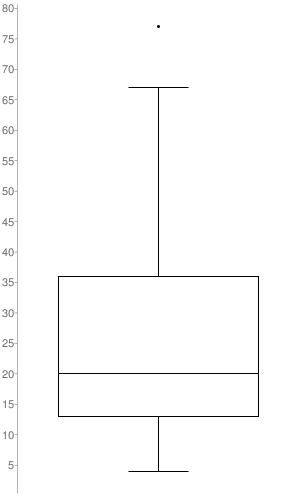
\includegraphics[width=0.6\textwidth]{picture/imagem1.png}
    \end{minipage}
    \begin{minipage}[H]{0.5\textwidth}
        \caption{Recuperação do Backend}
        \centering
        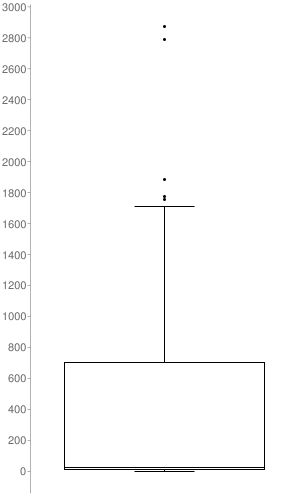
\includegraphics[width=0.6\textwidth]{picture/imagem2.png}
    \end{minipage}
\end{figure}

\begin{table}[H]
    \centering
    \caption{Recuperação do Frontend}
    \label{my-label}
    \begin{tabular}{|l|l|}
    \hline
    CATEGORIA     & VALOR      \\ \hline
    Média         & 26,87ms    \\ \hline
    Desvio Padrão & 17,42ms    \\ \hline
    População     & 45 unidades\\ \hline
    \end{tabular}
\end{table}

Estes dados são referentes a recuperação do serviço de leitura de requisições.

\begin{table}[H]
    \centering
    \caption{Recuperação do Backend}
    \label{my-label}
    \begin{tabular}{|l|l|}
    \hline
    CATEGORIA     & VALOR        \\ \hline
    Média         & 389,95ms     \\ \hline
    Desvio Padrão & 653,00ms     \\ \hline
    População     & 88 unidades  \\ \hline
    \end{tabular}
\end{table}

Estes dados são referentes a recuperação do serviço resolução de requisições.

\begin{figure}[H]
    \begin{minipage}[H]{0.5\textwidth}
        \caption{Solução Sem Erros}
        \centering
        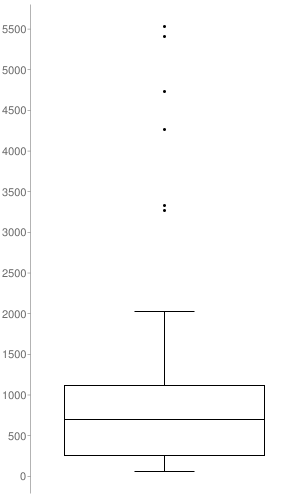
\includegraphics[width=0.6\textwidth]{picture/imagem4.png}
    \end{minipage}
    \begin{minipage}[H]{0.5\textwidth}
        \caption{Solução Final}
        \centering
        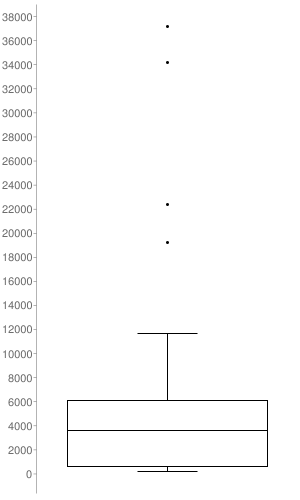
\includegraphics[width=0.6\textwidth]{picture/imagem3.png}
    \end{minipage}
\end{figure}    

\begin{table}[H]
    \centering
    \caption{Tempo de resposta da solução}
    \label{my-label}
    \begin{tabular}{|l|l|}
    \hline
    CATEGORIA     & VALOR        \\ \hline
    Média         & 893,49ms    \\ \hline
    Desvio Padrão & 906,98ms    \\ \hline
    População     & 148 unidades  \\ \hline
    \end{tabular}
\end{table}

Estes dados são referentes ao tempo de resposta de uma solução a qual não ocorre erros.

\begin{table}[H]
    \centering
    \caption{Tempo de resposta da solução ao usuário}
    \label{my-label}
    \begin{tabular}{|l|l|}
    \hline
    CATEGORIA     & VALOR        \\ \hline
    Média         & 5791,01ms    \\ \hline
    Desvio Padrão & 8426,14ms    \\ \hline
    População     & 41 unidades  \\ \hline
    \end{tabular}
\end{table}

Estes dados são referentes ao tempo de resposta a qual ocorrem erros no BackEnd.
\section{Conclusão}

Podemos observar que o tempo de recuperação do backend é muito mais crítico que o frontend, pois ao ocorrer um erro no backend é necessário recuperar toda a solução.O tempo de solução com os possíveis erros foi de até 10x o tempo de execução sem erros.

 Levantamos a hipótese de que se existisse uma gravação temporária da possível solução diminuiria significativamente o tempo de recuperação do backend.

\bibliographystyle{sbc}
\bibliography{sbc-template}

\end{document}
